% questions.tex —— 2005 年·普通高等学校招生考试·北京卷·文科 · 题目内容片段（无答案）
% 由 tools/generate_projects.py 依来源总账自 2005/2005_数学真题_北京文科_试题.md 生成，勿手改（改源 MD 后重跑）

\gkpart{一、选择题：本大题共 8 小题，每小题 5 分，共 40 分．在每小题给出的四个选项中，只有一项是符合题目要求的．}

\begin{question}
\gkti{1}设全集 $U = \mathbb{R}$，集合 $M = \{x \mid x > 1\}$，$P = \{x \mid x^2 > 1\}$，则下列关系中正确的是\mbox{（　　）}

\begin{gkopts}(2)
\task A．$M = P$
\task B．$P \subsetneqq M$
\task C．$M \subsetneqq P$
\task D．$M \cap P = \mathbb{R}$
\end{gkopts}

\end{question}
\begin{question}
\gkti{2}为了得到函数 $y = 2^{x-3} - 1$ 的图象，只需把函数 $y = 2^x$ 的图象上所有的点\mbox{（　　）}

\begin{gkopts}(1)
\task A．向右平移 3 个单位长度，再向下平移 1 个单位长度
\task B．向左平移 3 个单位长度，再向下平移 1 个单位长度
\task C．向右平移 3 个单位长度，再向上平移 1 个单位长度
\task D．向左平移 3 个单位长度，再向上平移 1 个单位长度
\end{gkopts}

\end{question}
\begin{question}
\gkti{3}“$m = \dfrac{1}{2}$”是“直线 $(m+2)x + 3my + 1 = 0$ 与直线 $(m-2)x + (m+2)y - 3 = 0$ 相互垂直”的\mbox{（　　）}

\begin{gkopts}(2)
\task A．充分必要条件
\task B．充分而不必要条件
\task C．必要而不充分条件
\task D．既不充分也不必要条件
\end{gkopts}

\end{question}
\begin{question}
\gkti{4}若 $|\vec{a}| = 1$，$|\vec{b}| = 2$，$\vec{c} = \vec{a} + \vec{b}$，且 $\vec{c} \perp \vec{a}$，则向量 $\vec{a}$ 与 $\vec{b}$ 的夹角为\mbox{（　　）}

\begin{gkopts}(4)
\task A．$30^\circ$
\task B．$60^\circ$
\task C．$120^\circ$
\task D．$150^\circ$
\end{gkopts}

\end{question}
\begin{question}
\gkti{5}从原点向圆 $x^2 + y^2 - 12y + 27 = 0$ 作两条切线，则这两条切线的夹角的大小为\mbox{（　　）}

\begin{gkopts}(2)
\task A．$\dfrac{\pi}{6}$
\task B．$\dfrac{\pi}{3}$
\task C．$\dfrac{\pi}{2}$
\task D．$\dfrac{2\pi}{3}$
\end{gkopts}

\end{question}
\begin{question}
\gkti{6}对任意的锐角 $\alpha, \beta$，下列不等关系中正确的是\mbox{（　　）}

\begin{gkopts}(1)
\task A．$\sin(\alpha + \beta) > \sin\alpha + \sin\beta$
\task B．$\sin(\alpha + \beta) > \cos\alpha + \cos\beta$
\task C．$\cos(\alpha + \beta) < \sin\alpha + \sin\beta$
\task D．$\cos(\alpha + \beta) < \cos\alpha + \cos\beta$
\end{gkopts}

\end{question}
\begin{question}
\gkti{7}在正四面体 $P - ABC$ 中，$D, E, F$ 分别是 $AB, BC, CA$ 的中点，下面四个结论中不成立的是\mbox{（　　）}

\begin{gkopts}(2)
\task A．$BC \parallel$ 平面 $PDF$
\task B．$DF \perp$ 平面 $PAE$
\task C．平面 $PDF \perp$ 平面 $ABC$
\task D．平面 $PAE \perp$ 平面 $ABC$
\end{gkopts}

\end{question}
\begin{question}
\gkti{8}五个工程队承建某项工程的 5 个不同的子项目，每个工程队承建 1 项，其中甲工程队不能承建 1 号子项目，则不同的承建方案共有\mbox{（　　）}

\begin{gkopts}(2)
\task A．$\mathrm{C}_4^1 \mathrm{C}_4^4$ 种
\task B．$\mathrm{C}_4^1 \mathrm{A}_4^4$ 种
\task C．$\mathrm{C}_4^4$ 种
\task D．$\mathrm{A}_4^4$ 种
\end{gkopts}

\end{question}
\gkpart{二、填空题：本大题共 6 小题，每小题 5 分，共 30 分．把答案填在横线上．}

\begin{question}
\gkti{9}抛物线 $y^2 = 4x$ 的准线方程是 \gkblank{}，焦点坐标是 \gkblank{}．

\end{question}
\begin{question}
\gkti{10}$\left(x - \dfrac{1}{x}\right)^6$ 的展开式中的常数项是 \gkblank{}．（用数字作答）

\end{question}
\begin{question}
\gkti{11}函数 $f(x) = \sqrt{x + 1} + \dfrac{1}{2 - x}$ 的定义域为 \gkblank{}．

\end{question}
\begin{question}
\gkti{12}在 $\triangle ABC$ 中，$AC = \sqrt{3}$，$\angle A = 45^\circ$，$\angle C = 75^\circ$，则 $BC$ 的长为 \gkblank{}．

\end{question}
\begin{question}
\gkti{13}对于函数 $f(x)$ 定义域中任意的 $x_1, x_2$ ($x_1 \neq x_2$)，有如下结论：

① $f(x_1 + x_2) = f(x_1) \cdot f(x_2)$；

② $f(x_1 \cdot x_2) = f(x_1) + f(x_2)$；

③ $\dfrac{f(x_1) - f(x_2)}{x_1 - x_2} > 0$；

④ $f\left(\dfrac{x_1 + x_2}{2}\right) < \dfrac{f(x_1) + f(x_2)}{2}$．

当 $f(x) = \lg x$ 时，上述结论中正确结论的序号是 \gkblank{}．

\end{question}
\begin{question}
\gkti{14}已知 $n$ 次多项式 $P_n(x) = a_0 x^n + a_1 x^{n-1} + \cdots + a_{n-1} x + a_n$．
如果在一种算法中，计算 $x_0^k$ ($k = 2, 3, 4, \cdots, n$) 的值需要 $k - 1$ 次乘法，计算 $P_3(x_0)$ 的值共需要 9 次运算（6 次乘法，3 次加法），那么计算 $P_{10}(x_0)$ 的值共需要 \gkblank{} 次运算．
下面给出一种减少运算次数的算法：$P_0(x) = a_0$，$P_{k+1}(x) = xP_k(x) + a_{k+1}$ ($k = 0, 1, 2, \cdots, n - 1$)．利用该算法，计算 $P_3(x_0)$ 的值共需要 6 次运算，计算 $P_{10}(x_0)$ 的值共需要 \gkblank{} 次运算．

\end{question}
\gkpart{三、解答题：本大题共 6 小题，共 80 分．解答应写出文字说明、证明过程或演算步骤．}

\begin{question}
\gkti{15}已知 $\tan\dfrac{\alpha}{2} = 2$，求：

(1) $\tan\left(\alpha + \dfrac{\pi}{4}\right)$ 的值；

(2) $\dfrac{6\sin\alpha + \cos\alpha}{3\sin\alpha - 2\cos\alpha}$ 的值．

\Needspace{0.4\textheight}
\end{question}
\begin{question}
\gkti{16}如图，在直三棱柱 $ABC - A_1B_1C_1$ 中，$AC = 3$，$BC = 4$，$AB = 5$，$AA_1 = 4$，点 $D$ 是 $AB$ 的中点．
\nopagebreak[4]
\begin{center}% Source-faithful schematic draft: 2005 Beijing Arts Q16, PDF p.1 (printed p.218).
% Source ID: src-fea4e73708ac3a85394b3698456c3244904a156c2ea4907c94a9bc9ed3e6cf8d
% Source SHA-256: 9ee1bf91b64cd5e48bd6415909f82ef61e023a117a843043c0ca22435102b3a1
\begin{tikzpicture}[line width=0.6pt, scale=0.95, every node/.style={inner sep=1.5pt}, baseline=(current bounding box.center)]
  % Coordinates of right triangular prism ABC-A1B1C1
  \coordinate (C) at (0, 0);
  \coordinate (A) at (-1.8, -1.0);
  \coordinate (B) at (2.2, -0.6);
  \coordinate (D) at ($(A)!0.5!(B)$);

  \coordinate (C1) at (0, 3.4);
  \coordinate (A1) at (-1.8, 2.4);
  \coordinate (B1) at (2.2, 2.8);

  % Dashed interior lines
  \draw[dashed, line width=0.5pt] (C) -- (A);
  \draw[dashed, line width=0.5pt] (C) -- (B);
  \draw[dashed, line width=0.5pt] (C) -- (C1);
  \draw[dashed, line width=0.5pt] (C) -- (D);
  \draw[dashed, line width=0.5pt] (C) -- (B1);
  \draw[dashed, line width=0.5pt] (A) -- (C1);
  \draw[dashed, line width=0.5pt] (B) -- (C1);

  % Solid exterior edges and lines
  \draw (A) -- (B);
  \draw (A) -- (A1);
  \draw (B) -- (B1);
  \draw (A1) -- (B1);
  \draw (A1) -- (C1);
  \draw (B1) -- (C1);
  \draw (D) -- (B1);

  % Labels
  \node[left] at (C) {$C$};
  \node[below left] at (A) {$A$};
  \node[below right] at (B) {$B$};
  \node[below] at (D) {$D$};
  \node[above] at (C1) {$C_1$};
  \node[left] at (A1) {$A_1$};
  \node[above right] at (B1) {$B_1$};
\end{tikzpicture}
\end{center}
\nopagebreak[4]
(1) 求证：$AC \perp BC_1$；

(2) 求证：$AC_1 \parallel$ 平面 $CDB_1$；

(3) 求异面直线 $AC_1$ 与 $B_1C$ 所成角的余弦值．

\end{question}
\begin{question}
\gkti{17}数列 $\{a_n\}$ 的前 $n$ 项和为 $S_n$，且 $a_1 = 1$，$a_{n+1} = \dfrac{1}{3}S_n$，$n = 1, 2, 3, \cdots$，求：

(1) $a_2, a_3, a_4$ 的值及数列 $\{a_n\}$ 的通项公式；

(2) $a_2 + a_4 + a_6 + \cdots + a_{2n}$ 的值．

\end{question}
\begin{question}
\gkti{18}甲、乙两人各进行 3 次射击，甲每次击中目标的概率为 $\dfrac{1}{2}$，乙每次击中目标的概率为 $\dfrac{2}{3}$．

(1) 甲恰好击中目标 2 次的概率；

(2) 乙至少击中目标 2 次的概率；

(3) 乙恰好比甲多击中目标 2 次的概率．

\end{question}
\begin{question}
\gkti{19}已知函数 $f(x) = -x^3 + 3x^2 + 9x + a$．

(1) 求 $f(x)$ 的单调减区间；

(2) 若 $f(x)$ 在区间 $[-2, 2]$ 上的最大值为 20，求它在该区间上的最小值．

\Needspace{0.4\textheight}
\end{question}
\begin{question}
\gkti{20}如图，直线 $l_1: y = kx$ ($k > 0$) 与直线 $l_2: y = -kx$ 之间的阴影区域（不含边界）记为 $W$，其左半部分记为 $W_1$，右半部分记为 $W_2$．
\nopagebreak[4]
\begin{center}% Source-faithful schematic draft: 2005 Beijing Arts Q20, PDF p.2 (printed p.219).
% Source ID: src-fea4e73708ac3a85394b3698456c3244904a156c2ea4907c94a9bc9ed3e6cf8d
% Source SHA-256: 9ee1bf91b64cd5e48bd6415909f82ef61e023a117a843043c0ca22435102b3a1
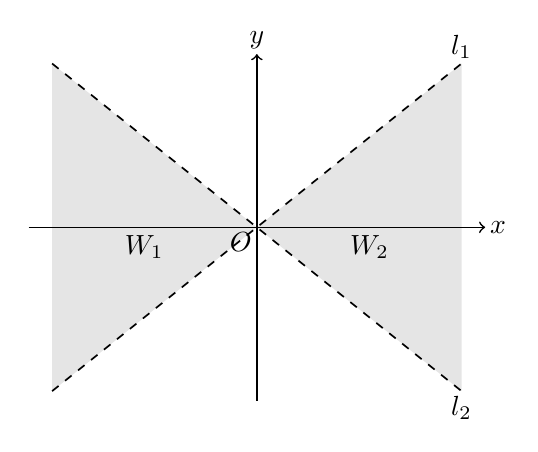
\begin{tikzpicture}[line width=0.6pt, scale=1.0, every node/.style={inner sep=1.5pt}, baseline=(current bounding box.center)]
  % Axes limits
  \def\xmax{2.6}
  \def\ymax{2.0}
  \def\k{0.8}

  % Shaded regions W1 and W2
  \fill[gray!20] (-\xmax, {-\k*\xmax}) -- (0, 0) -- (-\xmax, {\k*\xmax}) -- cycle;
  \fill[gray!20] (\xmax, {-\k*\xmax}) -- (0, 0) -- (\xmax, {\k*\xmax}) -- cycle;

  % Boundary dashed lines l1 and l2
  \draw[dashed, line width=0.6pt] (-\xmax, {-\k*\xmax}) -- (\xmax, {\k*\xmax}) node[above] {$l_1$};
  \draw[dashed, line width=0.6pt] (-\xmax, {\k*\xmax}) -- (\xmax, {-\k*\xmax}) node[below] {$l_2$};

  % Solid coordinate axes
  \draw[->] (-\xmax-0.3, 0) -- (\xmax+0.3, 0) node[right] {$x$};
  \draw[->] (0, -\ymax-0.2) -- (0, \ymax+0.2) node[above] {$y$};

  % Labels
  \node[below left] at (0, 0) {$O$};
  \node at ({-0.55*\xmax}, -0.25) {$W_1$};
  \node at ({0.55*\xmax}, -0.25) {$W_2$};
\end{tikzpicture}
\end{center}
\nopagebreak[4]
(1) 分别用不等式组表示 $W_1$ 和 $W_2$；

(2) 若区域 $W$ 中的动点 $P(x, y)$ 到 $l_1, l_2$ 的距离之积等于 $d^2$，求点 $P$ 的轨迹 $C$ 的方程；

(3) 设不过原点 $O$ 的直线 $l$ 与 (2) 中的曲线 $C$ 相交于 $M_1, M_2$ 两点，且与 $l_1, l_2$ 分别交于 $M_3, M_4$ 两点．求证：$\triangle OM_1M_2$ 的重心与 $\triangle OM_3M_4$ 的重心重合．

\end{question}